\chapter{Analysis and Design}
\section{Introduction}
This chapter presents the analysis and design of the proposed platform. It begins by identifying the functional and non-functional requirements that guide the system’s development. Then, it introduces the overall architecture and describes the different layers that structure the solution. Finally, it details the technologies selected for each component, along with the rationale behind these choices, in order to ensure scalability, reliability, and alignment with the project objectives.

\section{Requirements}
Defining the requirements of the platform is a crucial step to ensure that the proposed solution aligns with the project’s objectives. This section specifies both the functional requirements, which describe the essential services and capabilities the system must provide, and the non-functional requirements, which outline the quality attributes such as scalability, reliability, and performance. Together, they establish the foundation for the platform’s design and implementation.
\subsection{Functional Requirements}
The platform must provide the following core functionalities:
\begin{itemize}
\item \textbf{Infrastructure Provisioning:} The system should provide a robust, containerized, and orchestrated infrastructure capable of supporting real-time IoT data processing.
\item \textbf{Real-time Data Ingestion:} The platform must continuously collect and transmit data from IoT devices with low latency.
\item \textbf{Data Storage:} A scalable and reliable storage layer must be available to manage and store the high volume of data which is comming.
\item \textbf{Data Processing:} The system should process data in real time , enabling transformations, aggregations, and analytics.
\item \textbf{Monitoring and Visualization:} The platform must provide monitoring dashboards and visualization tools for IoT data streams and system health.
\item \textbf{Predictive Analytics:} The system should integrate AI/ML models (e.g., LSTM, GRU, GANs) for predictive maintenance, anomaly detection, and data augmentation.
\item \textbf{System Interaction:} Users must have access to a user-friendly interface to interact with the platform, query data, and extract insights.
\end{itemize}

\subsection{Non-Functional Requirements}
In addition to functionality, the platform must meet the following quality requirements:
\begin{itemize}
\item \textbf{Scalability:} The architecture should scale horizontally to support growing data volumes and devices.
\item \textbf{Reliability:} The platform must ensure fault tolerance, high availability, and consistency of services.
\item \textbf{Performance:} Data should be processed with low latency in real time pipeline..
\item \textbf{Maintainability:} The solution must be modular, allowing easy updates, debugging, and integration of new services.
\item \textbf{Portability:} The platform should run seamlessly in containerized environments in an on premise deployments.
\end{itemize}

\section{Architecture Design} 
\subsection{The infrastructure}
The foundation of the pipeline relies on a solid infrastructure that ensures the seamless integration of all its components. This infrastructure serves as the backbone that hosts and interconnects the different layers, guaranteeing scalability, resilience, and adaptability to evolving needs. Alongside, a dedicated monitoring and visualization environment is established to continuously track the system’s performance and health. This monitoring provides insights into data flows, processing efficiency, and potential anomalies, while visualization allows for an intuitive understanding of operational metrics. Together, these two aspects infrastructure and monitoring provide the stability and observability required for maintaining a reliable and efficient pipeline. 

\subsection{Pipeline Structure}

The foundation of the pipeline relies on a solid infrastructure that ensures the seamless integration of all its components. This infrastructure serves as the backbone that hosts and interconnects the different layers, guaranteeing scalability, resilience, and adaptability to evolving needs. Alongside, a dedicated monitoring and visualization environment is established to continuously track the system’s performance and health. This monitoring provides insights into data flows, processing efficiency, and potential anomalies, while visualization allows for an intuitive understanding of operational metrics. Together, these two aspects infrastructure and monitoring provide the stability and observability required for maintaining a reliable and efficient pipeline.

The pipeline itself is structured into four main layers, each addressing a specific stage in the data lifecycle:

\begin{itemize}
    \item \textbf{Data Generation:} Corresponds to the continuous production of information by IoT-like devices, generating data every 0.5 seconds.
    
    \item \textbf{Data Ingestion:} The layer where produced data is collected and funneled into the system in a consistent and reliable manner.
    
    \item \textbf{Data Processing:} Performs essential operations such as transformation, cleaning, and enrichment, ensuring that the data is accurate and usable for downstream tasks.
    
    \item \textbf{Data Storage:} Provides persistence with two sub-layers: one for storing daily operational data in a database for fast access, and another serving as a data lake to accumulate historical information for long-term analytics and exploration.
\end{itemize}
\begin{figure}[H]
    \centering
    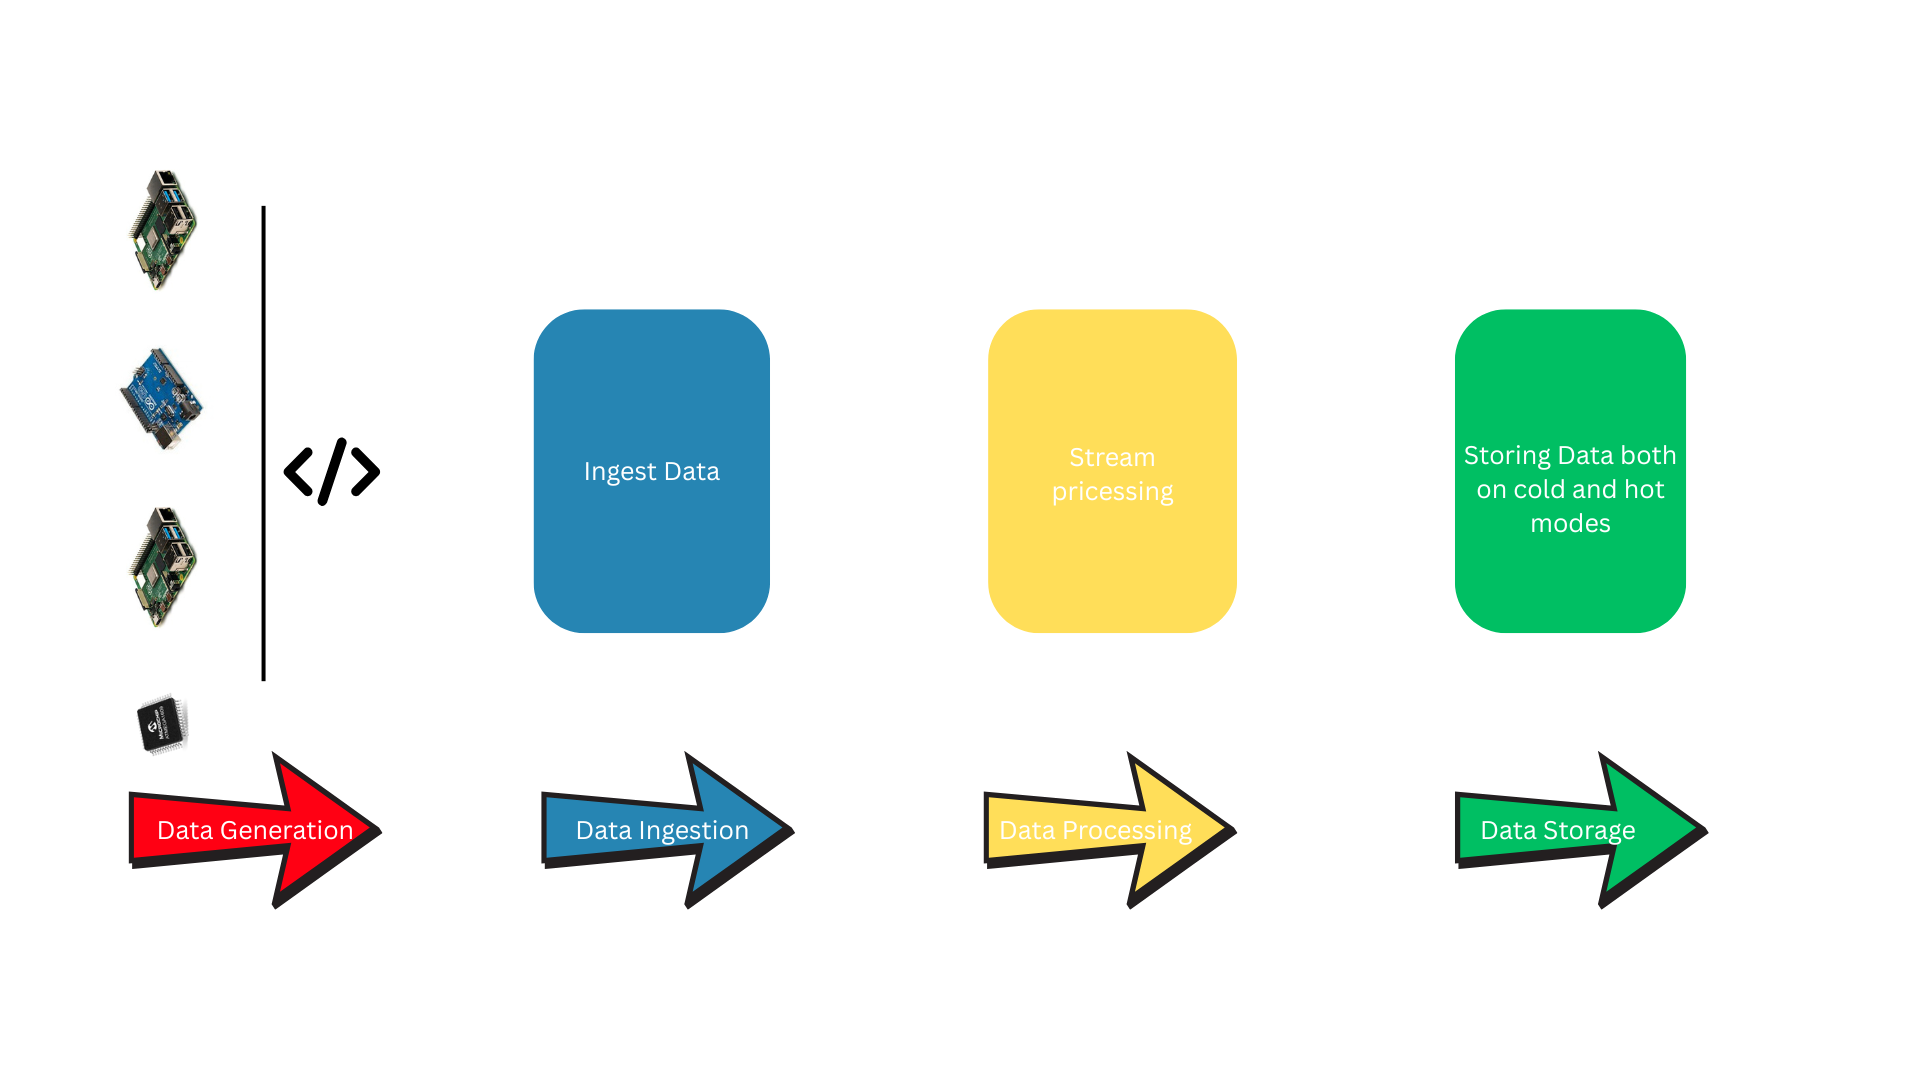
\includegraphics[width=0.8\textwidth]{images/architectureA.png}
    \caption{Architecture du pipeline}
\end{figure}

\subsection{Choice of Architecture}

For this project, the \textbf{Kappa architecture} was chosen as the most suitable approach. Unlike the Lambda architecture, which requires maintaining separate batch and streaming paths, Kappa simplifies the system by relying on a single streaming pipeline. This ensures reduced complexity, easier maintenance, and faster adaptability when changes are needed. Since the data is produced continuously every 0.5 seconds, a streaming oriented architecture like Kappa guarantees real time responsiveness while still allowing for reprocessing when necessary.

In addition to the streaming pipeline, a \textbf{cold storage layer based on a data lake } is integrated into the architecture. Data lakes provide a reliable, distributed, and scalable storage solution, which is essential for handling large volumes of historical data. This cold storage serves as the foundation for long term analytics, enabling retrospective insights and advanced exploration without compromising the performance of real time processing. The combination of Kappa with data lake thus ensures both immediate reactivity to live data and durable persistence for historical analysis, making it the best fit for the project’s requirements.

\section{Technological Stack}

The success of the proposed system relies heavily on the choice of technologies that ensure scalability, reliability, and performance. The technological stack is organized into four key domains: infrastructure, monitoring, data pipeline, and log management. Each domain is supported by specific tools chosen for their proven effectiveness in large-scale data-driven systems. 

\subsection{Infrastructure}

The infrastructure provides the foundation that supports the entire ecosystem. Several technologies are combined to achieve scalability, reproducibility, and automation:

\begin{itemize}
    \item \textbf{Terraform:} Used for Infrastructure as Code (IaC), Terraform allows us to provision and manage cloud or on-premise resources in a declarative manner. This ensures reproducibility of environments, simplifies scaling, and provides flexibility in adapting the infrastructure to evolving project requirements.
    \begin{figure}[H]
    \centering
    
\includegraphics[width=0.2\textwidth]{images/technologies/terraform.png}
    \caption{Terraform logo}
    \end{figure}
    
    \item \textbf{Ansible:} Complements Terraform by automating configuration management. While Terraform provisions resources, Ansible configures them by deploying dependencies and setting up environments, ensuring consistency across all nodes.
    
    \begin{figure}[H]
    \centering
    
\includegraphics[width=0.2\textwidth]{images/technologies/Ansible.png}
    \caption{Ansible logo}
    \end{figure}
    
    \item \textbf{Docker:} Ensures that all components of the system run in lightweight, isolated containers. This provides portability across different environments and eliminates compatibility issues, making the system easier to develop, test, and deploy.
      \begin{figure}[H]
    \centering
    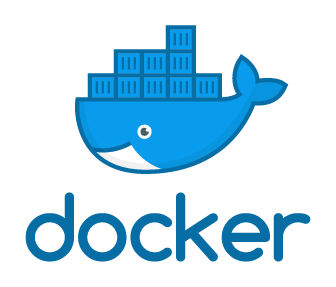
\includegraphics[width=0.2\textwidth]{images/technologies/docker.png}
    \caption{Docker logo}
    \end{figure}
    
    \item \textbf{Kubernetes (K3d):} K3d is a lightweight distribution of Kubernetes that runs Kubernetes clusters inside Docker. It is chosen for this project as it simplifies deployment, scaling, and orchestration of containerized applications while reducing overhead, making it ideal for development and testing environments.
    \begin{figure}[H]
    \centering
    
\includegraphics[width=0.2\textwidth]{images/technologies/Kubernetes.png}
    \caption{Kubernetes logo}
    \end{figure}
\end{itemize}

\subsection{Monitoring}

To guarantee reliability and performance, continuous monitoring of the system is essential. For this purpose, two complementary tools are employed:

\begin{itemize}
    \item \textbf{Prometheus:} A leading open-source monitoring system optimized for time-series data. It collects metrics from different components of the system, enabling alerting and real-time tracking of performance indicators such as latency, throughput, and system health.
         \begin{figure}[H]
    \centering
    
\includegraphics[width=0.2\textwidth]{images/technologies/Prometheus.png}
    \caption{Prometheus logo}
    \end{figure}
    \item \textbf{Grafana:} Provides powerful visualization capabilities, allowing collected metrics to be displayed through intuitive dashboards. By integrating with Prometheus, Grafana offers real-time insights into system behavior, enabling proactive decision-making and quick anomaly detection.
       \begin{figure}[H]
    \centering
    
\includegraphics[width=0.2\textwidth]{images/technologies/grafana.png}
    \caption{Grafana logo}
    \end{figure}
\end{itemize}

\subsection{Pipeline}

The pipeline represents the core of the project, managing the data lifecycle from ingestion to processing and storage:

\begin{itemize}
    \item \textbf{Zookeeper:} Provides coordination and synchronization for distributed systems, ensuring the reliability of Kafka by managing brokers and maintaining metadata consistency.
       \begin{figure}[H]
    \centering
    
\includegraphics[width=0.2\textwidth]{images/technologies/zookeeper.png}
    \caption{Apache Zookeeper logo}
    \end{figure}
    
    \item \textbf{Kafka:} Serves as the backbone for data ingestion and streaming. Its high throughput and fault tolerance make it the best fit for handling real-time data generated every 0.5 seconds, ensuring low-latency data delivery.
       \begin{figure}[H]
    \centering
    
\includegraphics[width=0.2\textwidth]{images/technologies/kafka.png}
    \caption{Apache Kafka logo}
    \end{figure}
    \item \textbf{Flink:} A robust stream processing engine designed for real-time analytics. Flink is chosen over alternatives due to its native support for event-time processing and fault-tolerant state management, which are critical for accurate and resilient stream processing.
       \begin{figure}[H]
    \centering
    
\includegraphics[width=0.2\textwidth]{images/technologies/flink.png}
    \caption{Apache Flink logo}
    \end{figure}
    
    \item \textbf{PostgreSQL:} Acts as the operational database for storing daily data. It combines reliability with strong support for structured queries, making it an excellent choice for fast access to recent information.
       \begin{figure}[H]
    \centering
    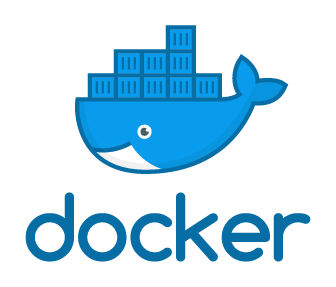
\includegraphics[width=0.2\textwidth]{images/technologies/docker.png}
    \caption{Docker logo}
    \end{figure}
    
    \item \textbf{HDFS:} Provides a distributed storage layer for historical data. HDFS is highly scalable and resilient, enabling the project to store vast amounts of data for long-term analysis.
       \begin{figure}[H]
    \centering
    
\includegraphics[width=0.2\textwidth]{images/technologies/hdfs.jpg}
    \caption{HDFS logo}
    \end{figure}
    \item \textbf{Hive:} Simplifies querying and analysis of the data stored in HDFS by providing a SQL-like interface. This bridges the gap between large-scale distributed storage and user-friendly analytics, enabling both technical and non-technical users to explore historical datasets efficiently
       \begin{figure}[H]
    \centering
    
\includegraphics[width=0.2\textwidth]{images/technologies/hive.png}
    \caption{Apache Hive logo}
    \end{figure}
\end{itemize}

\subsection{Log Management}

For comprehensive system observability, log management is implemented through the ELK stack:

\begin{itemize}
    \item \textbf{Elasticsearch:} Serves as a distributed search and analytics engine for storing logs. Its ability to handle large volumes of unstructured data makes it ideal for this project’s needs.
   \begin{figure}[H]
    \centering
    
\includegraphics[width=0.2\textwidth]{images/technologies/elastic.png}
    \caption{Elasticssearch logo}
    \end{figure}

    
    \item \textbf{Logstash:} Acts as the central pipeline for ingesting, transforming, and forwarding log data into Elasticsearch. This ensures that logs from different sources are consistently structured and indexed.
       \begin{figure}[H]
    \centering
    
\includegraphics[width=0.2\textwidth]{images/technologies/logstash.jpg}
    \caption{Logstash logo}
    \end{figure}
    \item \textbf{Kibana:} Provides visualization and exploration capabilities for the data stored in Elasticsearch. It allows developers and operators to analyze system behavior, detect anomalies, and troubleshoot issues effectively through dynamic dashboards.
       \begin{figure}[H]
    \centering
    
\includegraphics[width=0.2\textwidth]{images/technologies/kibana.png}
    \caption{Kibana logo}
    \end{figure}
\end{itemize}

\section{Technological Architecture}

The technological architecture of the project integrates a complete ecosystem of tools to manage the entire lifecycle of IoT data, from generation to visualization. As illustrated in Figure~\ref{fig:tech-arch}, the architecture is structured into interconnected layers: data ingestion, processing, storage, monitoring, and visualization. Each component plays a critical role in ensuring scalability, fault-tolerance, and real-time responsiveness. Infrastructure tools such as Terraform, Ansible, Kubernetes, and Docker provide a reliable foundation, while the pipeline leverages technologies like Kafka, Flink, PostgreSQL, and HDFS to handle data efficiently. Complementary components for monitoring (Prometheus, Grafana) and log management (ELK stack) ensure observability and system reliability. This modular design guarantees that the platform remains flexible and adaptable to evolving requirements.

\begin{figure}[H]
    \centering
    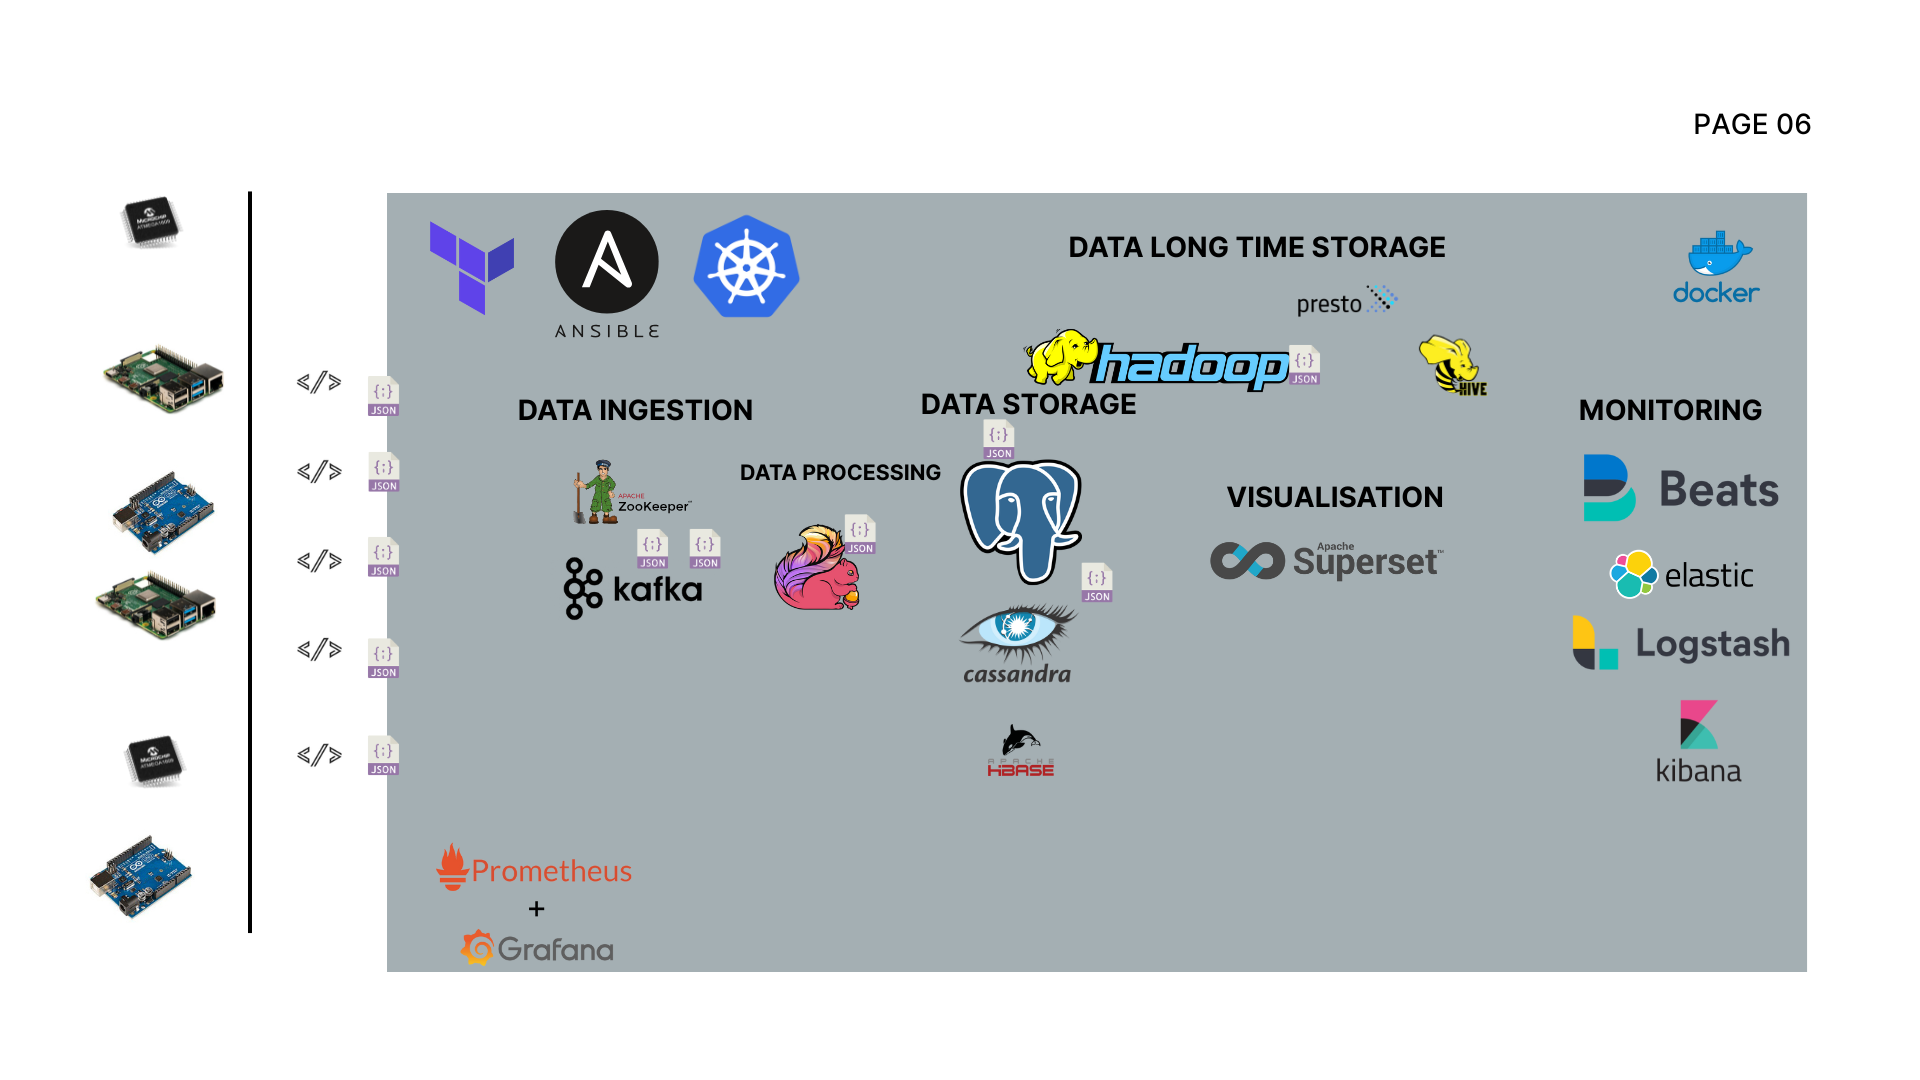
\includegraphics[width=\textwidth]{images/arch.png}
    \caption{Technological Architecture of the Project}
    \label{fig:tech-arch}
\end{figure}
